\chapter{Data processing}
\label{chap:processing}
\section{Epoching}

For each trial, we considered/filtered only the spikes that occurred 500 ms before the head-entry was detected--when infrared beam of the nosepoke was interrupted--and those up to when the head was moved out of the nosepoke. 

\begin{figure}
    \centering
    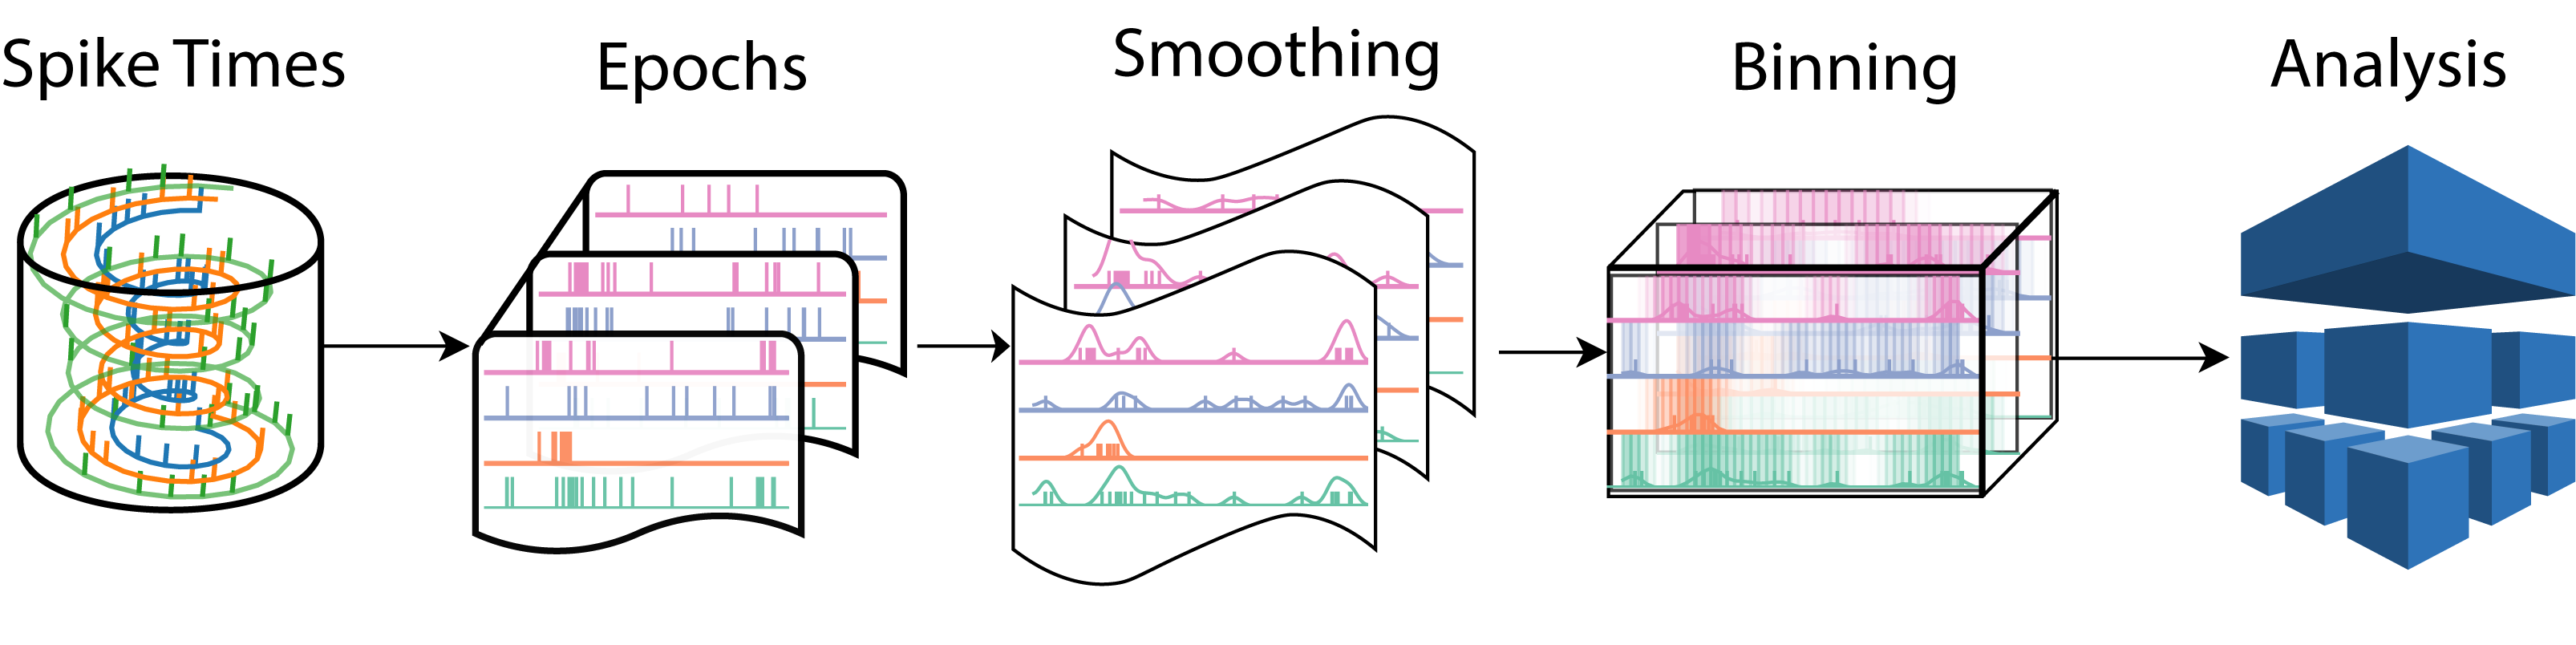
\includegraphics[width=\textwidth]{figures/Pipeline.png}
    \caption[Spike preprocessing steps]{Spike preprocessing steps: Spike times are epoched according to the nosepoke onsets, then smoothed to their estimated firing rate, and finally binned in equal-sized time bins, before being analyzed by machine learning. In the three middle steps we can see the activity of four neurons, in three different trials, through the preprocessing steps.}
    \label{fig:preproc}
\end{figure} 
% We divide spikes into their corresponding trials by using the events measured by our box. For each trial, we get all spikes that occurred between baseline (500ms before trial onset) and trial offset. This means it is possible to have the same spike in two trials, in cases when the intertrial interval is less than the baseline duration of 500ms, which was considered non-problematic.

% \subsection{Firing rate estimation}
% Before convolving we have to transform the time stamps into a boolean timeseries, for which we choose the precision of 1ms. Each neuron has then a time series of zeros and ones, with ones in times where the neuron was spiking.

\section{Firing Rate estimation}
We transformed the spike time-stamps into firing rates by convolving them with a \textit{kernel}. We used a gaussian kernel, for which we have to specify the standard deviation $\sigma$, which is the kernel width. We used three values for the standard deviation (20, 50 and 100), to assess the robustness of our analysis with respect to this parameter. To test the effects of different padding choices in estimating the firing rate, we compared the spike count (not smoothed) in 100ms bins with the firing rates measured using a gaussian kernel with standard deviation of 100ms, calculating the borders with either the default zero padding or a symmetric padding. At last we used the symmetric padding, to avoid creating temporal information which would appear in the case of zero padding.

% the precision is scaled down again by

% As we will hereafter compare data points, via measures of similarity and classification, we here describe in detail how they are represented.
After the convolution, we bin the spikes into windows of 100, 50 and 20 ms. While the windows of 100 and 50 can be used for computationally expensive analysis, The window of 20ms is stored for visualization purposes. For any given time bin we have activity in all measured neurons, represented by their instantaneous firing rate, yielding a vector of N dimensions, where N the number of neurons.

\section{Selection}
Engagement was assessed through the inter trial interval (ITI) of the animals. Since a single session can last more than a thousand trials, we expected that at some point the animal gets tired, in such a way that it may cease to engage in new trials immediately after the previous ones. We compared this interval between subsequent trials via visual inspection, and generously removed trials to be sure we wouldn't pollute posterior analysis with these unengaged trials.

Unless otherwise specified, we selected all correct trials (t > 1.5s) for our analysis, after the removal of trials without engagement. 
As typically done in the literature, we merged cells from all rats in most analysis, but we also performed these for each rat, to assess the consistency of our results. Each animal's first correct trial formed the first trial with increased number of (merged) cells, their second correct trial formed the second merged, and so on.

% For \ref{fig:behavior}, to show the animal learns, we plot the duration of each trial as the x-coordinate, as well as the walking average using a 100-trials window. We limit the xaxis to 3 seconds, although there were trials above this limit, to improve the visualization. We separe the selected trials into first and second half, and compare those using the probability density of response durations.%\todo{adicionar teste estatístico}

% To calculate the mean firing rate we selected all engaged trials with duration bigger than 1.5s, smoothed using either method, and then averaged the values between 0 and 1.5s along the trials. The result was shown for three trials in a single neuron, and for three neurons using the mean firing rate.